% !TeX root = ../libro.tex
% !TeX encoding = utf8


\chapter{Introducción}

\section{Introducción}

\noindent Actualmente, las \textbf{Redes Neuronales Convolucionales} (CNN\footnote{Convolutional Neural Network}) son una de las herramientas más usadas de la Inteligencia Artificial para tareas de Aprendizaje Automático (AA), de hecho son el principal objeto de estudio del \textbf{Deep Learning}, una subrrama del AA en la que hoy en día se está invirtiendo mucho esfuerzo en invesitgar y de la que anualmente se publican muchos artículos que nos enseñan la gran potencia de las CNN para diveras tareas.


\medskip

\noindent Destaca especialmente el excelente desempeño que tienen las CNN en el procesamiento de imágenes para tareas de clasificación, segmentación o incluso generación de nuevas imágenes. Es por ello que en el presente trabajo nos proponemos realizar una \textbf{modelización matemática} de estas CNN, para conocerlas mejor desde un punto de vista más teórico y \textbf{conocer algunas de sus principales propiedades} como la invarianza por traslaciones o frente a \entrecomillado{pequeñas} deformaciones. Finalmente, trataremos de \textbf{demostrar} la invarianza por traslaciones.

\medskip

\noindent En primer lugar vamos a definir el concepto de \textbf{Invarianza} como la capacidad de reconocer un objeto en una imagen incluso si su apariencia ha variado en algún sentido (mediante una rotación, una  ligera deformación o una traslación). Esto es algo muy importante, pues esto indica que se preserva la identidad del objeto incluso a pesar de haberse sometido a ciertos cambios.

\medskip

\noindent De esta forma definimos la \textbf{Invarianza por traslaciones} como la capacidad de reconocer la identidad de un objeto en una imagen incluso si este se ha desplazado. Esta propiedad es fundamental y sabemos que las CNN la verifican.

\begin{figure} [!h]
    \centering
    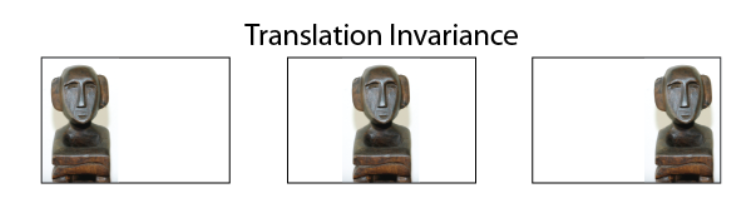
\includegraphics[width=0.8\textwidth]{img/translation_invariance.png}
    \caption{Las tres estatuas deben identificarse como iguales, aunque se ecuentren desplazadas.}
    \label{fig:invarianza_traslaciones}
\end{figure}

\medskip

\noindent Por otro lado, se conoce la \textbf{Invarianza frente a pequeñas deformaciones} (difeomorfismos) a la capacidad de reconocer la identidad de un objeto en una imagen a pesar de que este pueda haber sido alterado con pequeñas deformaciones.


\begin{figure}[!h]
  \centering
  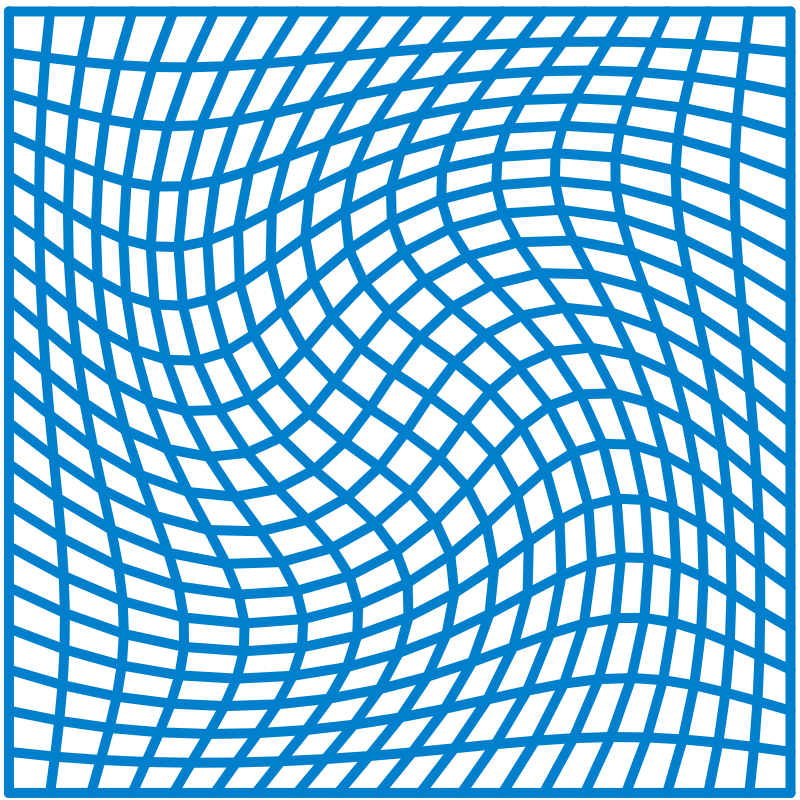
\includegraphics[width=0.5\textwidth]{img/Diffeomorphism.png}
  \caption{Acción de un difeomorfismo en una rejilla.}
  \label{fig:difeomorfismo}
\end{figure}

\begin{figure}[!h]
  \centering
  
\includegraphics[width=0.8\textwidth]{img/5_deformado.png}
  \caption{Todas las imágenes deberían clasificarse como 5, pese a las deformaciones.}
  \label{fig:deformaciones_5}
\end{figure}

\begin{figure}[!h]
  \centering
  
\includegraphics[width=0.5\textwidth]{img/1_excesivamente_deformado.png}
  \caption{Deformación excesiva que permite confundir el 1 con el 2 cuando se le aplica el difeomorfismo. Por eso nos centramos en \entrecomillado{pequeñas} deformaciones, para no alterar la identidad del objeto en la imagen.}
  \label{fig:deformaciones_1}
\end{figure}

\medskip


\noindent Esto motiva el estudio de las representaciones de traslaciones e invarianzas en las funciones de $L^2(\mathbb{R}^d)$, que son Lipschitz-continuas por la acción de difeomorfismos y que mantienen información de alta frecuencia para diferenciar entre distintos tipos de señales, con el objetivo de encontrar un operador que verifique todas estas propiedades y que presentaremos como la modelización matemática de una CNN.

\medskip

\noindent De esta manera, la invarianza por traslaciones, entendida en el contexto de las imágenes puede verse como trasladar cada pixel de la imagen en una misma dirección la misma distancia. En este sentido : 

\begin{definicion}
$L_cf(x)=f(x-c)$ es la traslación de $f \in L^2(\mathbb{R}^d)$ por $c \in \mathbb{R}^d$ .
\end{definicion}

\noindent Así, decimos que un operador $\Phi$ de  $L^2(\mathbb{R}^d)$ en un espacio de Hilbert $\mathcal{H}$ es invariante por traslaciones si $\Phi(L_cf(x))=\Phi(f)$ para todo $f \in L^2(\mathbb{R}^d)$ y para todo $c \in \mathbb{R}^d$. En el siguiente apartado trataremos el caso del módulo de la transformada de Fourier de $f$ como un ejemplo de un operador invariante por traslaciones. Sin embargo, es conocido el hecho de que aparecen inestabilidades frente a deformaciones en las altas frecuencias, y el mayor reto es preservar la Lipschitz-continuidad en esta situación.

\medskip

\noindent Para preservar la estabilidad en $L^2(\mathbb{R}^d)$ queremos que $\Phi$ sea no-expansiva. 

\begin{definicion}
Decimos que $\Phi$ es no-expansiva si: 
$$\forall (f,h) \in L^2(\mathbb{R}^d)^2 \; || \Phi(f)-\Phi(h)||_\mathcal{H} \leq ||f-h||$$
\end{definicion}

\noindent Por otro lado: 


\begin{definicion}
  Una función diferenciable $f: X \rightarrow \Omega$ dónde $X$ y $\Omega$ son variedades, es un \entrecomillado{Difeomorfismo} si $f$ es una biyección y su inversa $f^{-1}:\Omega \rightarrow X$ es también diferenciable. 
\end{definicion}


\noindent En nuestro caso, vamos a encargarnos de verificar la Lipschitz-continuidad relativa a la acción de pequeños difeomorfismos cercanos a las traslaciones. Dichos difeomorfismos transforman $x \in \mathbb{R}^d$ en $x-\tau (x)$ dónde $\tau$ es el campo de desplazamiento. 

\begin{definicion}
Denotemos $L_{\tau} f(x)=f(x-\tau(x))$ como la acción del difeomorfismo $\mathbb{1}-\tau$ en $f$.
\end{definicion} 

\medskip

\noindent Por otro lado, la condición de Lipschitz es la siguiente: 

\begin{definicion}
  Sea $f: M \rightarrow N$ una función entre dos espacios métricos $M$ y $N$ con sus respectivas distancias $d_M$ y $d_N$. Se dice que $f$ satisface la condición de Lipschitz si $\exists C>0$ tal que: 

  $$d_N(f(x),f(y))\leq C d_M(x,y), \; \; \forall x,y \in M$$
\end{definicion}

\noindent En nuestro caso, la $d_N$ que utilizaremos será la norma del espacio de Hilbert $\mathcal{H}$ de llegada, pero necesitamos definir de alguna manera una distancia $d_M$ entre los difeomorfismo $\mathbb{1}$ y $\mathbb{1}-\tau$ para escribir correctamente la condición de Lipschitz. Además, dado que el espacio de partida es $L^2(\mathbb{R}^d)$ y los puntos que vamos a comparar son las funciones $f$ y $L_\tau f=f(x-\tau(x))$ sabemos que $\|\Phi(f) - \Phi(L_cf) \|$ estará acotada por $\|f\| · d(\mathbb{1}, \mathbb{1}-\tau)$, de manera que necesitamos definir una distancia entre el difeomorfismo $\mathbb{1}$ y $\mathbb{1}-\tau$. Para ello, la topología débil \footnote{ recordemos que es la topología menos fina de un espacio normado que hace continuas todas las aplicaciones de su dual} en los difeomorfismos $C^2$  permite definir la siguiente aplicación, que utilizaremos como distancia:

\begin{definicion}
Así, se define una distancia entre $\mathbb{1}-\tau$ y $\mathbb{1}$ en cualquier subconjunto compacto $\Omega$ de $\mathbb{R}^d$ como 

\begin{equation} \label{eq::distancia}
  d_\Omega(\mathbb{1},\mathbb{1}-\tau) = \sup_{x \in \Omega} |\tau (x)| + \sup_{x \in \Omega} |\nabla \tau (x)| + \sup_{x \in \Omega}|H \tau (x)|
\end{equation}

\end{definicion}
\medskip

\noindent Dónde $|\tau (x)|$ es la norma euclídea en $\mathbb{R}^d$, $\nabla |\tau (x)|$ la norma del supremo de la matriz $\nabla \tau (x)$, y $|H \tau (x)|$ la norma del supremo del Hessiano.

\medskip

\noindent Así, podemos finalmente expresar la condición de Lipschitz que un operador debería satisfacer en nuestro caso:  

\medskip

\begin{definicion} \label{def::Lipschitz_cont}
\noindent Un operador invariante por traslaciones $\Phi$ se dice \entrecomillado{Lipchitz-continuo} por la acción de los difeomorfismos $C^2$  si para cualquier compacto $\Omega \subset \mathbb{R}^d$ existe una constante $C$ tal que para todo $f \in L^2(\mathbb{R}^d)$ con Soporte en $\Omega$ y para todo $\tau \in C^2(\mathbb{R}^d)$ se cumple:

\begin{equation} \label{eq::Lipschitz_condition}
  || \Phi(f)-\Phi(L_{\tau}f)||_\mathcal{H} \leq C||f||(\sup_{x \in \mathbb{R}^d} |\nabla \tau (x)| + \sup_{x \in \mathbb{R}^d}|H \tau (x)|)
\end{equation}
con  $|| \nabla \tau ||_\infty + ||H \tau ||_\infty < 1$ para asegurarnos de que la deformación sea invertible \cite{doi:10.1137/S0036141002404838}.
\end{definicion}

\medskip

\noindent Debido a que $\Phi$ es invariante a traslaciones, la cota superior de Lipschitz no depende de la amplitud máxima de traslación $\sup_{x \in \mathbb{R}^d}|\tau (x)|$ de la métrica del difeomorfismo \eqref{eq::distancia}. Por otro lado la continuidad Lipschitz de \eqref{eq::Lipschitz_condition} implica que $\Phi$ es invariante por traslaciones globales, pero es mucho más fuerte. $\Phi$ se ve poco afectada por los términos de primer y segundo grado de difeomorfismos que son traslaciones locales.

\medskip


\noindent Una vez presentadas las principales herramientas con las que trabajaremos, en las futuras secciones veremos como para la elección de ciertos operadores como el módulo de la transformada de Fourier existen problemas para satisfacer la condición de Lipschitz en altas frecuencias. Para solucionar el problema se optará por utilizar transformadas de ondeletas, pero esto abre nuevos problemas como serán el hecho de que no son invariantes por traslaciones. Por ello será necesario componer la transformada con un operador no lineal que será el módulo para obtener coeficientes invariantes por traslaciones. Este nuevo operador que consistirá en una cascada de convoluciones de operadores no lineales y no conmuntativos de manera que cada uno de ellos calcula el módulo de la transfomada de odeletas, y será este nuevo operador el que podremos interpretar como la modelización matemática de una CNN.

\subsection{Notación}

\begin{itemize}
    \item $|| \tau ||_\infty := \sup_{x \in \mathbb{R}^d} |\tau(x)|$
    \item $||\nabla \tau ||_\infty := \sup_{x \in \mathbb{R}^d} |\nabla \tau(x)|$
    \item $||\mathcal{H} \tau ||_\infty := \sup_{x \in \mathbb{R}^d} |\mathcal{H} \tau(x)|$ dónde $|\mathcal{H} \tau(x)|$ es la norma del tensor Hessiano. 
    \item La norma en $L^2(\mathbb{R}^d)$ de $f$ lo denotamos $||f||$.
    \item La norma de $f$ en $L^1(\mathbb{R}^d)$ lo denotamos $||f||_1=\int{|f(x)| dx}$.
    \item Se denota $g \circ f(x)=f(gx)$ a la acción de un elemento del grupo $g\in G$.
    \item Un operador  $\mathcal{R}$ parametrizado por $p$ es denotado por $\mathcal{R}[p]$ y $\mathcal{R}[\Omega]=\lbrace \mathcal{R}[p] \rbrace_{p \in \Omega}$. 
\end{itemize}




\endinput
